\documentclass[compress]{beamer}
\usepackage{ifthen,verbatim}

\title{Alignment Status and Plans}
\author{Jim Pivarski, Alexei Safonov, K\'aroly Banicz$^*$}
\institute{Texas A\&M University, $^*$FermiLab}
\date{27 March, 2008}

\newcommand{\isnote}{}
\xdefinecolor{lightyellow}{rgb}{1.,1.,0.25}
\xdefinecolor{darkblue}{rgb}{0.1,0.1,0.7}

%% Uncomment this to get annotations
%% \def\notes{\addtocounter{page}{-1}
%%            \renewcommand{\isnote}{*}
%% 	   \beamertemplateshadingbackground{lightyellow}{white}
%%            \begin{frame}
%%            \frametitle{Notes for the previous page (page \insertpagenumber)}
%%            \itemize}
%% \def\endnotes{\enditemize
%% 	      \end{frame}
%%               \beamertemplateshadingbackground{white}{white}
%%               \renewcommand{\isnote}{}}

%% Uncomment this to not get annotations
\def\notes{\comment}
\def\endnotes{\endcomment}

\setbeamertemplate{navigation symbols}{}
\setbeamertemplate{headline}{\mbox{ } \hfill
\begin{minipage}{5.5 cm}
\vspace{-0.75 cm} \small
\end{minipage} \hfill
\begin{minipage}{4.5 cm}
\vspace{-0.75 cm} \small
\begin{flushright}
\ifthenelse{\equal{\insertpagenumber}{1}}{}{Jim Pivarski \hspace{0.2 cm} \insertpagenumber\isnote/\pageref{numpages}}
\end{flushright}
\end{minipage}\mbox{\hspace{0.2 cm}}\includegraphics[height=1 cm]{../cmslogo} \hspace{0.1 cm} \includegraphics[height=1 cm]{../tamulogo} \hspace{0.01 cm} \vspace{-1.05 cm}}

\begin{document}
\frame{\titlepage}

%% \begin{notes}
%% \item This is the annotated version of my talk.
%% \item If you want the version that I am presenting, download the one
%% labeled ``slides'' on Indico (or just ignore these yellow pages).
%% \item The annotated version is provided for extra detail and a written
%% record of comments that I intend to make orally.
%% \item Yellow notes refer to the content on the {\it previous} page.
%% \item All other slides are identical for the two versions.
%% \end{notes}


\begin{frame}
\frametitle{Outline and Scope}
\begin{itemize}\setlength{\itemsep}{0.5 cm}
\item General plan and where we are now
\item Timeline in detail
\begin{itemize}\setlength{\itemsep}{0.25 cm}
\item Updated software/scripts
\item Track-cut study
\item CSC overlap procedure
\item iCSA08 and pre-CSA08
\item CRA0T/CRAFT and beam-halo
\end{itemize}
\item Database monitoring tools
\end{itemize}

\vfill \small
($\sim$15-minute talk)
\end{frame}

% Timeline
% * March:
%   1. infrastructure for comparing (and maybe manually changing) muon geometry in database: done two days ago, needs to be documented/publicized
%   2. back-port last HIP-related software updates to 1_6_7 to develop procedure with existing MC samples
%   3. implement first draft of a HIP alignment procedure with CSC overlap hits and pass it to Karoly for development on beam-halo
%   * develop DQM alignment validation
% * April:
%   * optimize large-dataset procedure with new track cut
%   * possibly hybrid procedure with overlap hits in CSCs
%   * determine expected performance with 0~T and 3.8~T cosmic rays
%   * apply to CRA0T dataset if that would be interesting
%   * develop database monitoring plots
%   * determine expected performance of CSC overlap method with beam-halo
%     * apply ``beam-halo'' procedure to nearly horizontal MTCC muons
% * May:
%   * Do systematics studies on re-optimized procedure, startup procedures, cosmic ray tests
%   * Update expected effect of misalignment on muon tracks, physics quantities
%   * apply procedure to CRAFT dataset
%     * compare with hardware measurements
% * June:
%   * use beam-halo tracks to align endcap chambers, possibly layers
%     * compare and/or combine with hardware measurements
% * July:
%   * align large structures with first 1000 tracks
%   * combine measurements (beam-halo, CRAFT, first 1000 tracks, hardware measurements, etc.)
% * and beyond:
%   * apply full-scale procedure

\begin{frame}
\frametitle{General plan}

\mbox{\hspace{-0.75 cm} 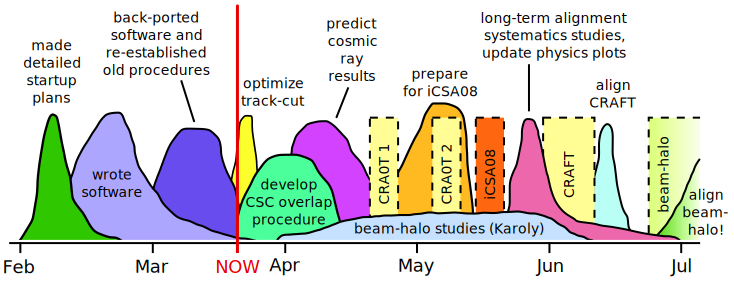
\includegraphics[width=1.12\linewidth]{plan.png}}

\small
\begin{itemize}
\item \textcolor{darkblue}{Done:} software preparation and updating old scripts
\item \textcolor{darkblue}{This month:} incorporate track-cut, develop start-up procedures
\item \textcolor{darkblue}{May:} iCSA08 preparation and execution
\item \textcolor{darkblue}{June:} systematics studies, physics plots (POG), and CRAFT
\item \textcolor{darkblue}{July:} beam-halo, hopefully!
\end{itemize}
\end{frame}

\begin{frame}
\frametitle{Software and scripts 1}

\small
\begin{itemize}\setlength{\itemsep}{0.3 cm}
\item Developed everything for 2\_0\_X (on time!)
\begin{itemize}\setlength{\itemsep}{0.1 cm}
\item Mostly moving minor tools from private directories to official infrastructure
\item e.g.\ alignable CSC rings, track cut, APE interface, new plots
\item Also HLT/AlCaRECO paths for beam-halo data stream
\end{itemize}

\item Private 1\_6\_7 back-port to access old event samples
\begin{itemize}\setlength{\itemsep}{0.1 cm}
\item Track-fitting with CSC overlap hits
\item All the new alignment 2\_0\_X features and interface \\ (to ease transition to real 2\_0\_X)
\end{itemize}

\item Helped with official 1\_8\_X back-port, to be used in pre-CSA08 test
\begin{itemize}\setlength{\itemsep}{0.1 cm}
\item Will include a special stream with CSC overlap hits
\end{itemize}
\end{itemize}
\end{frame}

\begin{frame}
\frametitle{Software and scripts 2}

\small
\begin{itemize}\setlength{\itemsep}{0.2 cm}
\item Updated 100~pb$^{-1}$ alignment script to use new interface
\item Applied track-cut, well into automated alignment procedure \\ (after some false starts)
\end{itemize}
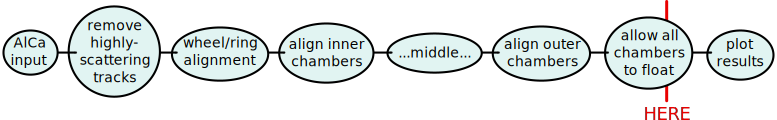
\includegraphics[width=\linewidth]{drawing.png}

\begin{center}
\includegraphics[width=0.6\linewidth]{cafplot.png}
\end{center}
\end{frame}

\begin{frame}
\frametitle{Track-cut study: old results}

\vspace{-0.5 cm}
\begin{center}
\begin{tabular}{p{0.45\linewidth} p{0.45\linewidth}}
\begin{center}Baseline procedure w/o cut\end{center} & \begin{center}Quick track-cut test\end{center}
\end{tabular}

\vspace{-0.5 cm}
\includegraphics[width=5. cm, angle=90]{convergence-100.pdf}
\includegraphics[width=5. cm, angle=90]{large_APEs_trackcut-100.pdf}

\small (Each line is a station's resolution as a function of iteration)
\end{center}

\small
\vspace{-0.25 cm}
\begin{itemize}
\item Dramatic improvement in one iteration
\item But this is not an apples-to-apples comparison
\item Want to do the whole procedure with pre-selected tracks
\end{itemize}
\end{frame}

\begin{frame}
\frametitle{CSC overlap procedure}

\begin{itemize}
\item Align CSC chambers relative to each other in each ring
\item Originally considered for beam-halo alignment, but it could be
just as useful for I.P. tracks (especially low-energy tracks)
\item Layer alignment is similar, but doesn't need overlaps
\item Event samples:

\vspace{0.25 cm}
\mbox{\small
\hspace{-1.5 cm} \begin{tabular}{c c c p{0.43\linewidth}}
Overlaps in $W\to\mu\nu$ & 1\_6\_7 & re-fit tracks & for developing procedure, can get started soon \\
Overlaps in beam-halo & 1\_6\_7 & re-fit tracks & realistic studies (Karoly) \\
Overlaps in min-bias $\mu$ & 1\_8\_X & pre-iCSA08 & realistic studies, iCSA08 prep \\
Overlaps in soup & 2\_0\_X & iCSA08 & realistic studies \\
\end{tabular}}

\end{itemize}

\vfill
\uncover<2>{\hspace{-0.83 cm} \textcolor{darkblue}{\Large Predicting cosmic ray results}

\begin{itemize}
\item Baseline procedure with track cut for several chambers
\item In time to make a decision about aligning CRA0T
\begin{itemize}
\item Would an alignment without a $p_T$ cut yield interesting results?
\end{itemize}
\end{itemize}

\mbox{\small
\hspace{-0.85 cm} \begin{tabular}{c c c c}
Underground cosmics with and without $\vec{B}$ & 1\_6\_7 & on tape & realistic studies \\
\end{tabular}}}
\end{frame}

\begin{frame}
\frametitle{iCSA08}

\begin{itemize}\setlength{\itemsep}{0.35 cm}
\item It's a timed test and very public
\begin{itemize}
\item Need to get it right the first time!
\end{itemize}
\item Pre-CSA08 provides approximately the same samples in 1\_8\_X
\item Planned muon alignment procedures:
\begin{enumerate}\setlength{\itemsep}{0.15 cm}
\item Baseline with high $p_T$ and track cut \hfill (test with $W$ sample)
\item CSC overlap alignment within rings, followed by ring alignment \\ \hfill (test with min-bias)
\item CSC layer alignment \hfill (test with min-bias)
\item CSC beam-halo if it's ready \hfill (no 1\_8\_X test available)
\end{enumerate}
\end{itemize}

\vfill
\uncover<2>{\hspace{-0.83 cm} \textcolor{darkblue}{\Large Systematics studies and physics plots}
\begin{itemize}
\item Repeat of old studies with re-optimized procedure
\item Can use 1\_6\_7 samples, 1\_8\_X overlaps, and iCSA08 soup
\end{itemize}}
\end{frame}

\begin{frame}
\frametitle{CRAFT (and maybe CRA0T)}
\begin{center}
\includegraphics[width=0.6\linewidth]{craft.pdf}
\end{center}

\small
\vspace{-0.75 cm}
\begin{itemize}
\item Baseline procedure on top and bottom chambers
\begin{itemize}
\item in muon barrel (1 million muons through tracker?)
\item possibly as far out as ME1/3 (10k muons?)
\end{itemize}
\end{itemize}

\hspace{-0.83 cm} \textcolor{darkblue}{\Large Followed soon afterward by CSC beam-halo alignment}
\begin{itemize}
\item Complete coverage of ring 1, possibly ring 2, but not ME1/3
\end{itemize}
\end{frame}

%% \begin{frame}
%% \frametitle{Outline}
%% \begin{itemize}\setlength{\itemsep}{0.75 cm}
%% \item 
%% \end{itemize}
%% %% \hspace{-0.83 cm} \textcolor{darkblue}{\Large Outline2}
%% \end{frame}

%% \section*{First section}
%% \begin{frame}
%% \begin{center}
%% \Huge \textcolor{blue}{First section}
%% \end{center}
%% \end{frame}

\begin{frame}
\frametitle{Database monitoring tools}

\begin{itemize}
\item Motivating problem: CMSSW can't read multiple alignments from the database (with the same IOV) in one job
\item Solution: convert database records into intermediary files
\item Generalized conversion procedure so that everyone can use it
\end{itemize}

\vspace{-0.25 cm}
\begin{center}
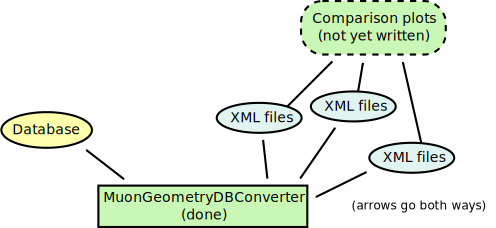
\includegraphics[width=0.7\linewidth]{geometryconversion.png}
\end{center}

\vspace{-0.25 cm}
\begin{itemize}
\item Samir is already using this tool to upload DCOPS measurements to the database
\item I'm writing comparison plots on an as-needed basis
\end{itemize}
\end{frame}

\begin{frame}
\frametitle{Conclusions}
\begin{itemize}
\item Mostly about scheduling, so I'll re-draw the timeline
\end{itemize}

\vfill
\mbox{\hspace{-0.75 cm} 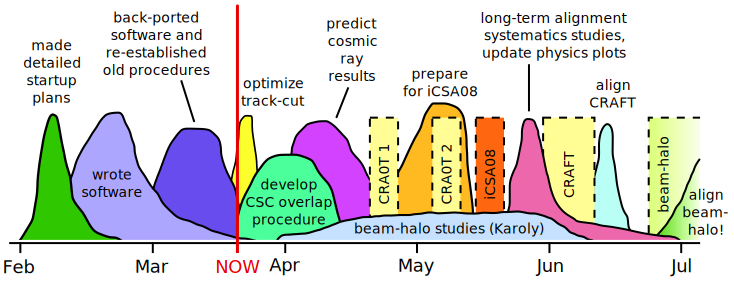
\includegraphics[width=1.12\linewidth]{plan.png}}

\vfill
\begin{itemize}
\item No time devoted exclusively to comparison-plot development
\begin{itemize}
\item Can be split into a separate project, if there is someone who would like to work on it
\item Groundwork has been laid, scope is well-defined
\end{itemize}
\end{itemize}

\label{numpages}
\end{frame}

\end{document}
